
\chapter{Sprint 0}
\label{Sprint0}
\lhead{Chapter 6. \emph{Sprint 0}}

\section{Duration}
The duration of the sprint was the following:
\begin{itemize}
\item Sprint start: August, 26th
\item Sprint end: September, 8th
\end{itemize}

\section{Planning}

Our first sprint was focused on project planning and preliminary studies.
We planned to receive some kind of approval on our understanding of the project
as described by the customer before starting preliminary studies. This was done mainly to avoid
\begin{enumerate}[a)]
\item planning a solution for a different problem and
\item wasting resources studying something that would not be relevant for the project.
\end{enumerate}
In an effort to prepare a draft of system requirements to be approved by the customer,
we planned some brainstorming sessions to pin down a number candidates for health measurements
(weight, blood pressure\ldots) to be supported by the system.

\section{Goal(s)}

We wanted to achieve a sufficient understanding of the problem's scope,
relevant technologies and similar solutions as well as:% complete a high-level planning which would have included:
\begin{enumerate}[a)]
\item identify high-level requirements, phases and milestones
\item identify a high-level system architecture
\item choose a development process
\end{enumerate}

Additionally, we wanted to decide what software to use to write the report,
choose and setup development enviroments, SDKs and version control systems in order to be able
to get going with development and documentation as soon as necessary.

\begin{figure}[h]
\centering
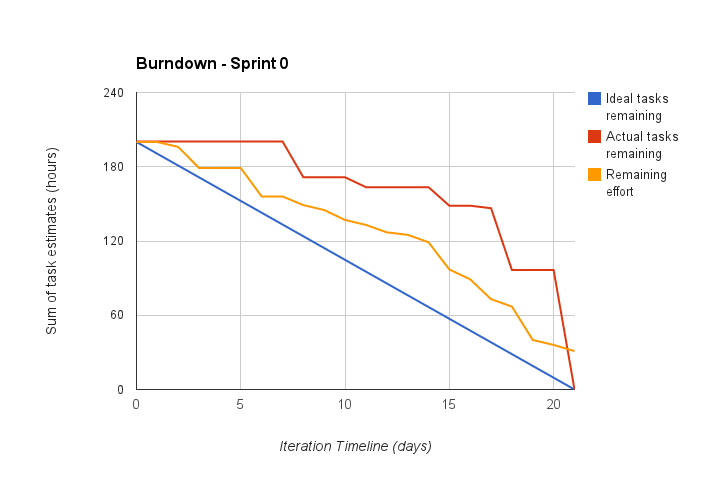
\includegraphics[scale=0.60]{../Figures/burndownSprint0.png}
\caption{Burndown chart Sprint 0}
\label{figure:burndownsprint0}
\end{figure}

\newpage
\section{Backlog}

See below the sprint backlog.
\begin{enumerate}[1.]
	\item \textbf{Project planning} for this sprint included:
		\begin{itemize}
			\item \textbf{Booking of rooms}:
				where to hold meetings and work.
			\item \textbf{Scheduling weekly meetings}:
				with both the customer and supervisor.
			\item \textbf{Choice of development process}:
				candidates are Waterfall and Scrum.
			\item \textbf{Requirements gathering}:
				an initial set (draft) of high-level requirements.
			\item \textbf{Risk analysis}:
				a first draft.
		\end{itemize}
	\item \textbf{Project management} included:
		\begin{itemize}
			\item \textbf{Sprint startup meeting}:
				included sprint planning and review
			\item \textbf{Weekly meetings}:
				with both customer and supervisor (from the 26th).
			\item \textbf{Meeting notes}:
				taking notes during meetings, reviewing of the notes.
			\item \textbf{Status reports}:
				for weeks 35 and 36.
		\end{itemize}
	\item \textbf{Read course's compendium}
	\item \textbf{Preliminary studies}\newline
		of relevant technologies like databases, web-servers and web APIs.
	\item \textbf{Identify possibile measurements}\newline
		to be supported by the system (glucose, weight\ldots).
	\item \textbf{Preliminary system architecture}\newline
		brainstorm on a high-level architecture to be submitted to the client for feedback.
	\item \textbf{Choice and setup of project's tools}\newline
		such as tools for the report and version control system.
	\item \textbf{Android environment setup}\newline
		both IDEs and SDK.
	\item \textbf{Group dynamics lecture}\newline
		attendance is mandatory.
\end{enumerate}


\section{Results and feedback}

\begin{figure}[h]
\centering
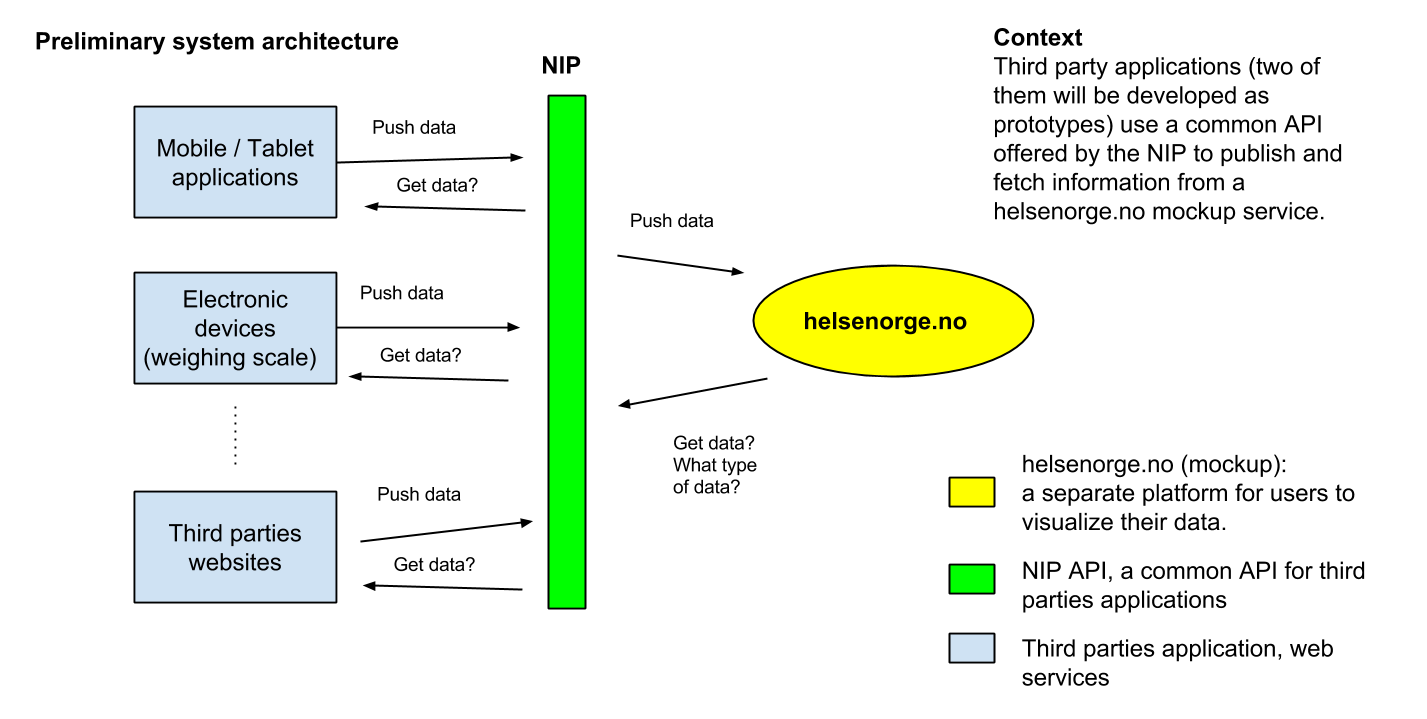
\includegraphics[scale=0.30]{../Figures/architecture-draft.png}
\caption{System architecture (draft)}
\label{figure:architecture-draft}
\end{figure}

During the first days of the project, which were technically not part of any sprint,
we met each other, the customer and the supervisor.
The customer described the problem, explaining what he had in mind and why it was relevant for him.
The supervisor handed us some notes to help the project kick-off.
We exchanged contacts information (both mail and Skype) to make sure everybody could reach out to
everybody else. Additionally, we set up a Facebook group where to post relevant informations
and a Google Drive folder to share and collaborate on editing documents.
We scheduled weekly meetings with all involved parties as follows:
\begin{itemize}
\item customer and supervisor meetings on Mondays
\item collective work sessions on Mondays (10.00 - 19.00) and Wednesdays (15.00 - 19.00)
\end{itemize}

At the beginning of the sprint we shared our thoughts on what we had understood from the customer.
In order to ensure we had a proper understanding of the problem we produced a diagram
(figure \ref{figure:architecture-draft}) representing a high-level architecture
of the product (an \textit{ehealth integration platform}) and submitted it to the customer
via mail for feedback.

It consisted of:
\begin{enumerate}[1.]
\end{enumerate}

We then begun studying relevant technologies and similar solutions and eventually identified
a number of candidate health measurements and submitted those to the customer as well.

Our idea was to develop three prototype applications, other than the integration
platform and front-end, to be able to demonstrate how these systems interoperate.
Each of these prototypes would have focused on a single health measurement.

We found an agreement with the customer on heart rate and weight measurements which we had
proposed based on two facts. Firstly, we had found an open-source Android application which could
measure the user's heart rate using the mobile's camera and hoped we could use it for one prototype.
Secondly, one team member owned a Withings weighing scale device which we tought
would be interesting to use for another prototype.
The customer agreed on these candidates because they were two of the most common measurements.

A possible third application was discussed both internally and with the customer but
given time and resource constraints of this project we intentionally left it rather vague
as we were unsure whether we would have had time for that.

By the end of the sprint the customer started mentioning Microsoft's HealthVault and suggesting
that some kind of interoperability with HealthVault would have proved valuable for him.

With regards of our development process, we decided to use Scrum based on various considerations as
described in \ref{section:development-methodology}. To better perform Scrum, we decided
to use an online tool called \textit{Scrumdo}, described in section \ref{section:tools}.
We also chose and setup other tools like:
\begin{itemize}
\item version control system (Git and GitHub)
\item development environment (IntelliJ IDEA)
\item documentation (LaTeX)
\end{itemize}

\section{Evaluation}

%The sprint generally achieved its expected results.
At the end of the sprint we had achieved a good understanding of the problem and a good overview on a
high-level system architecture and requirements. We didn't get as far as we hoped on our studies on some particular
technologies and this was due to a number of factors. Firstly, estimating the amount of time required to obtain
a sufficient knowledge in a topic resulted difficult and we generally needed more time than we thought and had planned.
Secondly, we had little familiarity with most involved technologies.
Given the size of our group, we had some difficulties mitigating this problem due to
our reduced technical skill pool. Some difficult topics of study were Apache Camel, its extension Apache IPF,
and whether it was desiderable to use these instead of the Spring framework (and why).
Although by the end of the sprint we came to an agreement on what technologies we need to use
(database, web server\ldots) we didn't decide on a specific implementation of such technologies
(Apache Tomcat, Spring, Apache Camel, JAX-RS\ldots).

During this sprint we did not manage to send all the documents the supervisor
required or they were missing some important detail. However, what we sent
was sufficient to give him a good understanding of our progress so we
consider this a minor issue.
